% Op icon: parametric curve — a sine hump closed by its chord into a lightly filled face, with the parameter axis dashed.
\documentclass[tikz,border=2mm]{standalone}
\usetikzlibrary{arrows.meta,calc,shapes.geometric}
\begin{document}
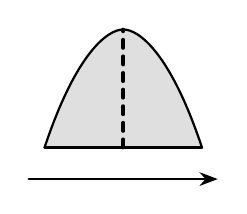
\begin{tikzpicture}[line width=1.3pt, line cap=round, line join=round, >=Stealth, x=1mm,y=1mm]
  \fill[gray!25] (-10,-6) .. controls (-6,6) and (-2,9) .. (0,9) .. controls (2,9) and (6,6) .. (10,-6) -- cycle;
  \draw[thick] (-10,-6) .. controls (-6,6) and (-2,9) .. (0,9) .. controls (2,9) and (6,6) .. (10,-6);
  \draw[thick] (-10,-6) -- (10,-6);
  \draw[dashed] (0,-6) -- (0,9);
  \draw[thick, ->] (-12,-10) -- (12,-10);
\end{tikzpicture}
\end{document}
